\documentclass[border=15pt, multi, tikz]{standalone}
%\usepackage{blocks}
\usepackage{import}
\subimport{../../layers/}{init}
\usetikzlibrary{positioning}
\usetikzlibrary{3d} %for including external image 

\def\ConvColor{rgb:yellow,5;red,2.5;white,5}
\def\ConvReluColor{rgb:yellow,5;red,5;white,5}
\def\PoolColor{rgb:red,1;black,0.3}
\def\FcColor{rgb:blue,5;red,2.5;white,5}
\def\FcReluColor{rgb:blue,5;red,5;white,4}
\def\SoftmaxColor{rgb:magenta,5;black,7}

\begin{document}
\begin{tikzpicture}
\tikzstyle{connection}=[ultra thick,every node/.style={sloped,allow upside down},draw=\edgecolor,opacity=0.7]
%%%%%%%%%%%%%%%%%%%%%%%%%%%%%%%%%%%%%%%%%%%%%%%%%%%%%%%%%%%%%%%%%%%%%%%%%%%%%%%%%%%%%%%%
%% Draw Layer Blocks
%%%%%%%%%%%%%%%%%%%%%%%%%%%%%%%%%%%%%%%%%%%%%%%%%%%%%%%%%%%%%%%%%%%%%%%%%%%%%%%%%%%%%%%%
\node[canvas is zy plane at x=0] (temp) at (-3,0,0) {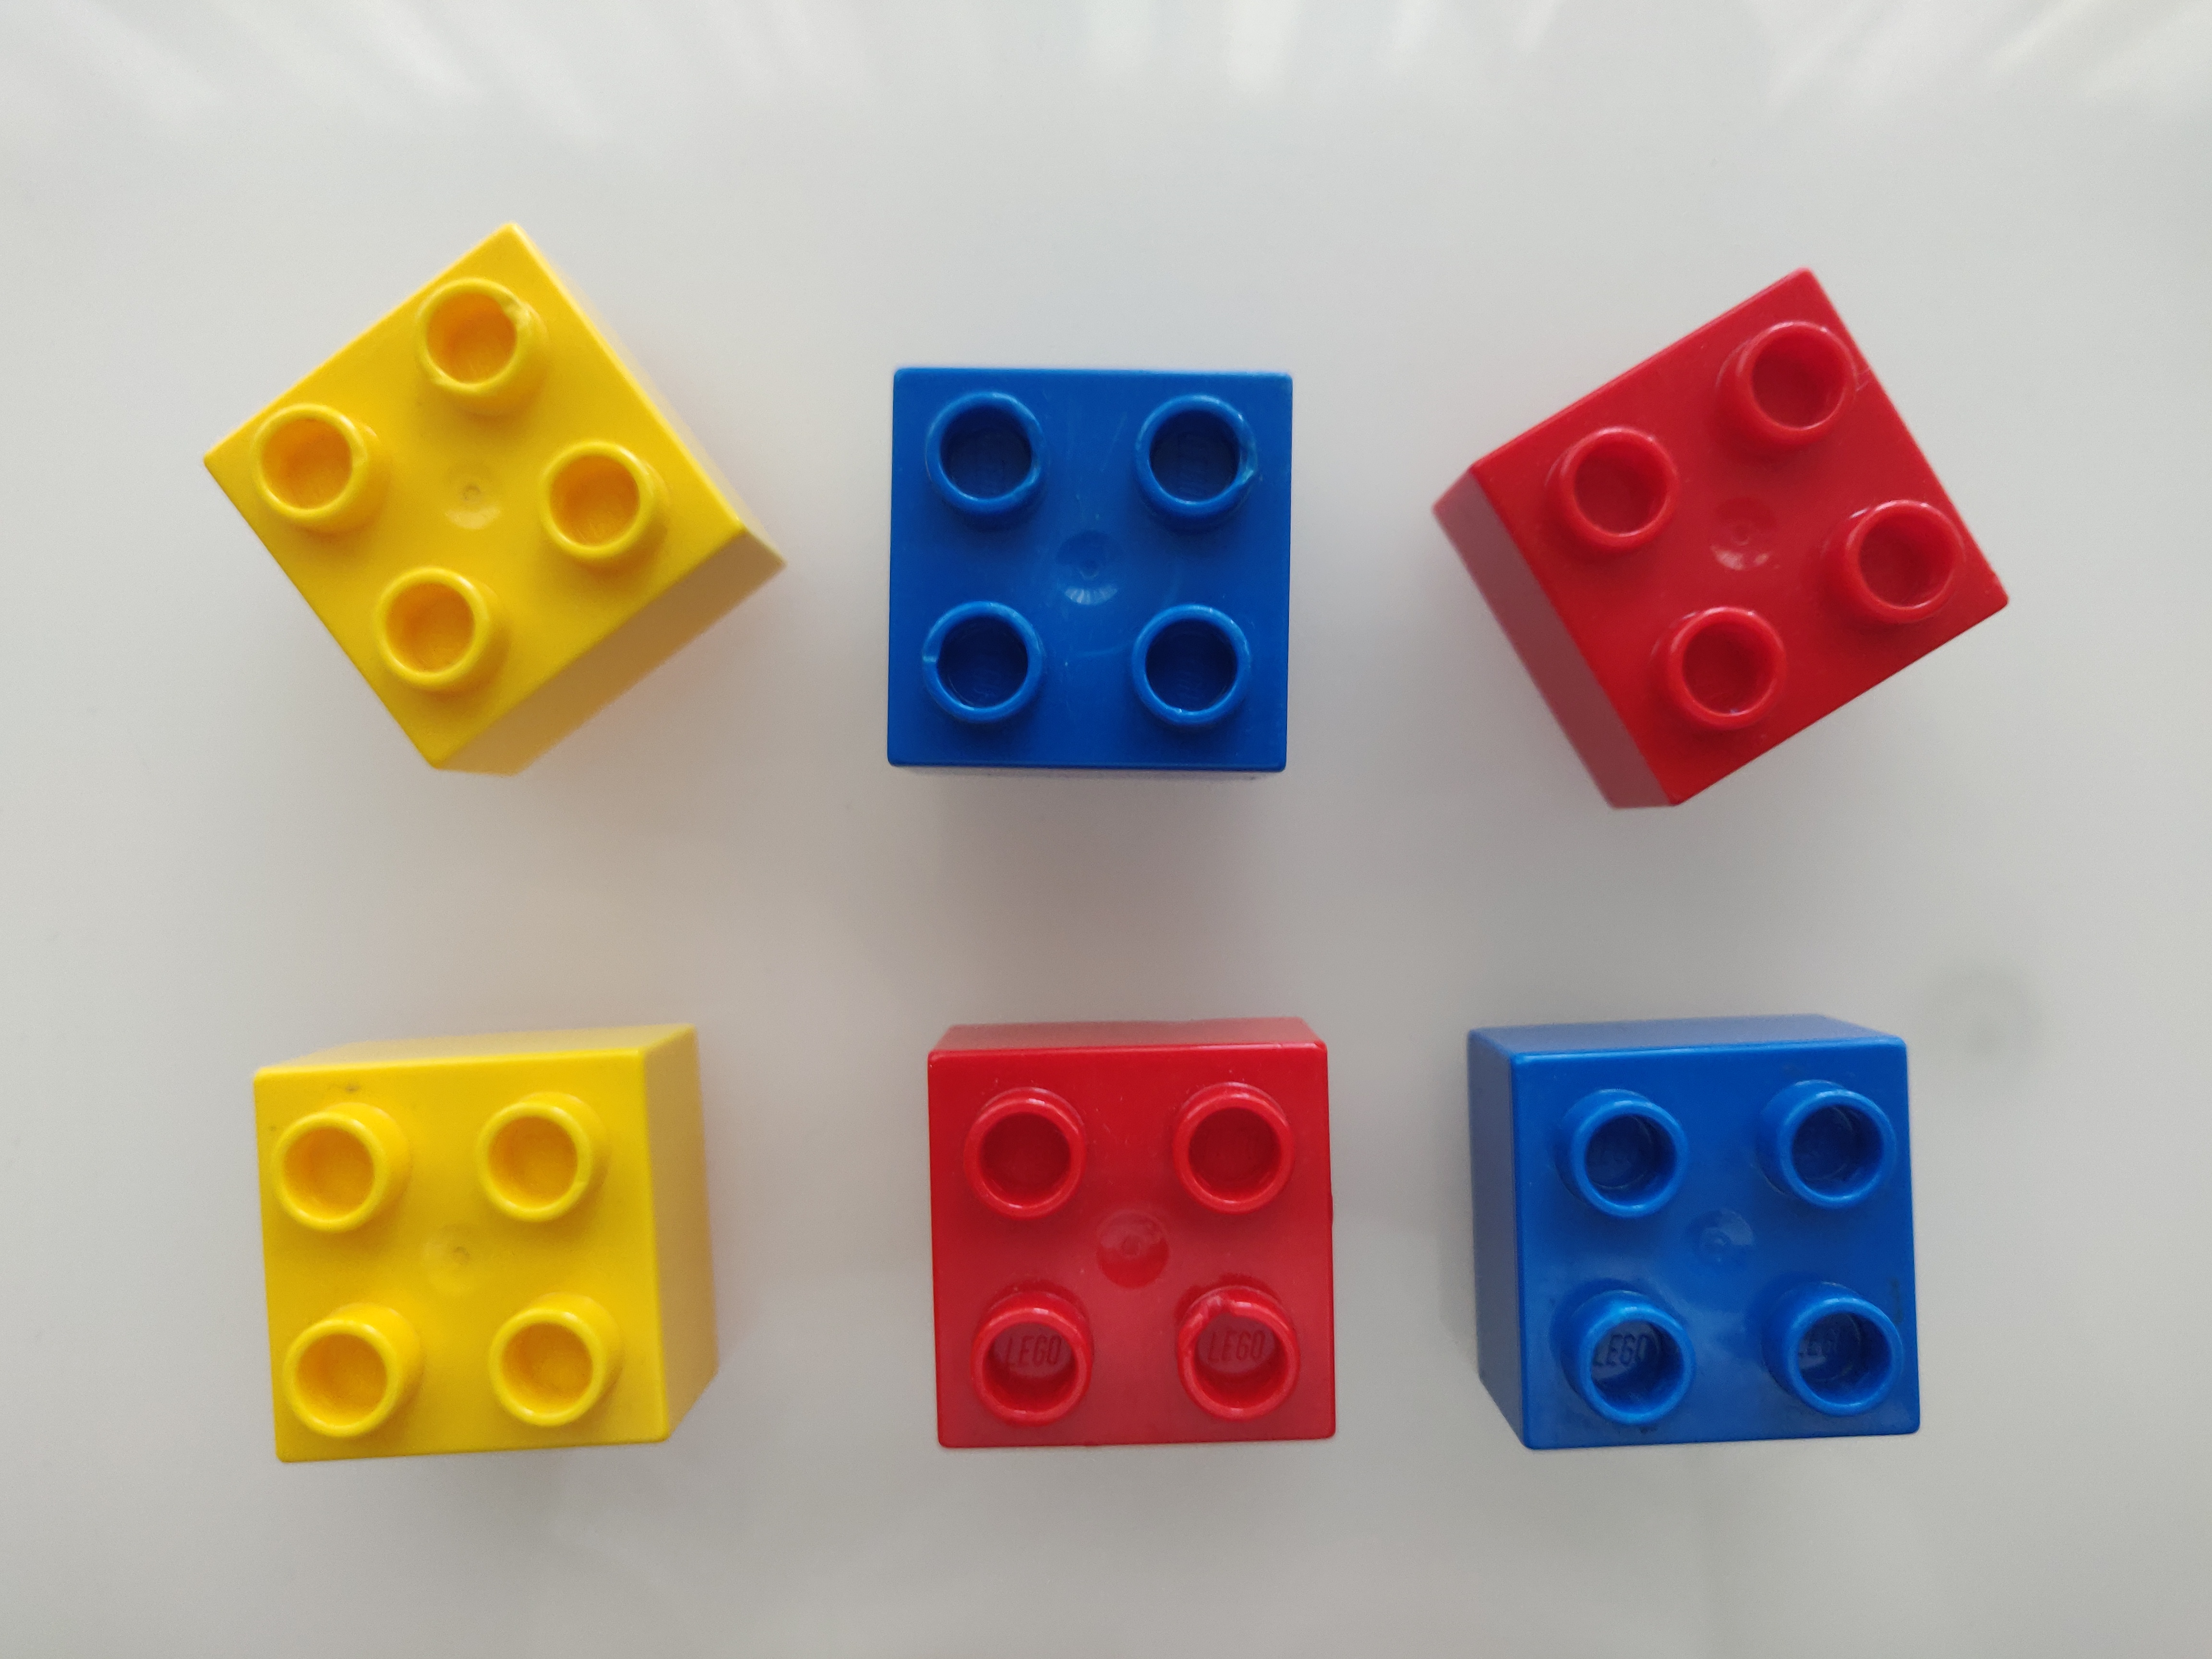
\includegraphics[width=8cm,height=8cm]{LEGO.jpg}};
% conv1
\pic[shift={(0,0,0)}] at (0,0,0) {RightBandedBox={name=cr1,caption=conv1,%
        xlabel={{"96","dummy"}},ylabel=,zlabel=55,fill=\ConvColor,bandfill=\ConvReluColor,%
        height=40,width={2},depth=40}};
%pool1
\pic[shift={(0,0,0)}] at (cr1-east) {Box={name=p1,%
        fill=\PoolColor,opacity=0.5,height=35,width=1,depth=35}};
%%%%%%%%%%
% conv2
\pic[shift={(2,0,0)}] at (p1-east) {RightBandedBox={name=cr2,caption=conv2,%
        xlabel={{"256","dummy"}},ylabel=27,zlabel=27,fill=\ConvColor,bandfill=\ConvReluColor,%
        height=25,width={5},depth=25}};
%pool2
\pic[shift={(0,0,0)}] at (cr2-east) {Box={name=p2,%
        fill=\PoolColor,opacity=0.5,height=20,width=1,depth=20}};
%%%%%%%%%%
% conv3
\pic[shift={(2,0,0)}] at (p2-east) {RightBandedBox={name=cr3,caption=conv3,%
        xlabel={{"384","dummy"}},ylabel=13,zlabel=13,fill=\ConvColor,bandfill=\ConvReluColor,%
        height=15,width={8},depth=15}};
%pool3
\pic[shift={(0,0,0)}] at (cr3-east) {Box={name=p3,%
        fill=\PoolColor,opacity=0.5,height=10,width=1,depth=10}};
%%%%%%%%%%
% conv4
\pic[shift={(1.8,0,0)}] at (p3-east) {RightBandedBox={name=cr4,caption=conv4,%
        xlabel={{"384","dummy"}},ylabel=13,zlabel=13,fill=\ConvColor,bandfill=\ConvReluColor,%
        height=15,width={8},depth=15}};
%pool4
\pic[shift={(0,0,0)}] at (cr4-east) {Box={name=p4,%
        fill=\PoolColor,opacity=0.5,height=10,width=1,depth=10}};
%%%%%%%%%%
% conv5
\pic[shift={(1.5,0,0)}] at (p4-east) {RightBandedBox={name=cr5,caption=conv5,%
        xlabel={{"256","dummy"}},ylabel=13,zlabel=13,fill=\ConvColor,bandfill=\ConvReluColor,%
        height=15,width={8},depth=15}};
%pool5
\pic[shift={(0,0,0)}] at (cr5-east) {Box={name=p5,%
        fill=\PoolColor,opacity=0.5,height=10,width=1,depth=10}};
%%%%%%%%%%
% fc6
\pic[shift={(3,0,0)}] at (p5-east) {RightBandedBox={name=fc6,caption=fc6,%
        xlabel={{"1","dummy"}},ylabel=1,zlabel=4096,fill=\FcColor,bandfill=\FcReluColor,%
        height=3,width=3,depth=100}};
%%%%%%%%%%
% fc7
\pic[shift={(2,0,0)}] at (fc6-east) {RightBandedBox={name=fc7,caption=fc7,%
        xlabel={{"1","dummy"}},ylabel=1,zlabel=4096,fill=\FcColor,bandfill=\FcReluColor,%
        height=3,width=3,depth=100}};
%%%%%%%%%%
% fc8
\pic[shift={(1.5,0,0)}] at (fc7-east) {RightBandedBox={name=fc8,caption=fc8+regression,%
        xlabel={{"1","dummy"}},ylabel=1,fill=\FcColor,bandfill=\FcReluColor,%
        height=3,width=3,depth=5}};

%%%%%%%%%%
% regression
\pic[shift={(0,0,0)}] at (fc8-east) {Box={name=regression,%
        xlabel={{"","dummy"}},zlabel=1,opacity=0.8,fill=\SoftmaxColor,%
        height=3,width=1.5,depth=5}};
    
%%%%%%%%%%%%%%%%%%%%%%%%%%%%%%%%%%%%%%%%%%%%%%%%%%%%%%%%%%%%%%%%%%%%%%%%%%%%%%%%%%%%%%%%
%% Draw Arrow Connections
%%%%%%%%%%%%%%%%%%%%%%%%%%%%%%%%%%%%%%%%%%%%%%%%%%%%%%%%%%%%%%%%%%%%%%%%%%%%%%%%%%%%%%%%
\draw [connection]  (p1-east)        -- node {\midarrow} (cr2-west);
\draw [connection]  (p2-east)        -- node {\midarrow} (cr3-west);
\draw [connection]  (p3-east)        -- node {\midarrow} (cr4-west);
\draw [connection]  (p4-east)        -- node {\midarrow} (cr5-west);
\draw [connection]  (p5-east)        -- node {\midarrow} (fc6-west);
\draw [connection]  (fc6-east)       -- node {\midarrow} (fc7-west);
\draw [connection]  (fc7-east)       -- node {\midarrow} (fc8-west);
\draw [connection]  (regression-east)   -- node {\midarrow} ++(1.5,0,0);
%%%%%%%%%%%%%%%%%%%%%%%%%%%%%%%%%%%%%%%%%%%%%%%%%%%%%%%%%%%%%%%%%%%%%%%%%%%%%%%%%%%%%%%%
%% Draw Dotted Edges 
%%%%%%%%%%%%%%%%%%%%%%%%%%%%%%%%%%%%%%%%%%%%%%%%%%%%%%%%%%%%%%%%%%%%%%%%%%%%%%%%%%%%%%%%
\draw[densely dashed]
    (fc6-west)++(0, 1.5*.2, 1.5*.2) coordinate(a) -- (p5-nearnortheast)
    (fc6-west)++(0,-1.5*.2, 1.5*.2) coordinate(b) -- (p5-nearsoutheast)
    (fc6-west)++(0,-1.5*.2,-1.5*.2) coordinate(c) -- (p5-farsoutheast)
    (fc6-west)++(0, 1.5*.2,-1.5*.2) coordinate(d) -- (p5-farnortheast)
    
    (a)--(b)--(c)--(d)
    ;
%%%%%%%%%%%%%%%%%%%%%%%%%%%%%%%%%%%%%%%%%%%%%%%%%%%%%%%%%%%%%%%%%%%%%%%%%%%%%%%%%%%%%%%%
\end{tikzpicture}
\end{document}
